\section{Resultados}

Neste capítulo são apresentados os resultados dos métodos propostos nesta dissertação. Primeiramente, é apresentado os resultados do primeiro método de segmentação e, também, os resultados encontrados pela aplicação da rede neural convolucional YOLO. Posteriormente, é apresentado os resultados do segundo método de segmentação. Por fim, é apresentada uma comparação entre os dois métodos de segmentação utilizando a métrica IoU.

\subsection{PRIMEIRO MÉTODO DE SEGMENTAÇÃO}

A seguir, serão apresentados os resultados obtidos pelo primeiro método de segmentação. As figuras \ref{fig:controle-yolo-primeira}, \ref{fig:controle-yolo-segunda}, \ref{fig:tw-yolo-primeira}, \ref{fig:tw-yolo-segunda}, \ref{fig:ct-yolo-primeira}, \ref{fig:ct-yolo-segunda}, \ref{fig:twt-yolo-primeira} e \ref{fig:twt-yolo-segunda} ilustra imagens depois da aplicação da rede neural YOLO. Já as figuras \ref{fig:controle-seg-primeira}, \ref{fig:controle-seg-segunda}, \ref{fig:tw-seg-primeira}, \ref{fig:tw-seg-segunda}, \ref{fig:ct-seg-primeira}, \ref{fig:ct-seg-segunda}, \ref{fig:twt-seg-primeira} e \ref{fig:twt-seg-segunda} ilustram o resultado final do primeiro método de segmentação.

\subsubsection{CONTROLE}

\begin{figure}[!h]
    \centering
    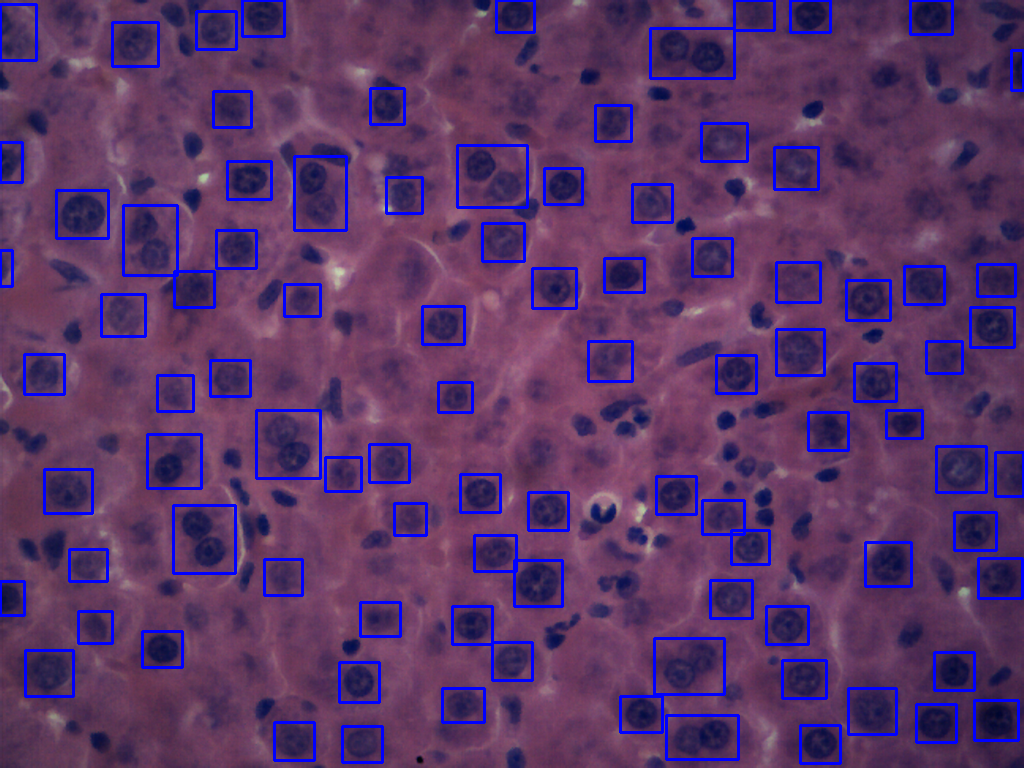
\includegraphics[width = 13cm, height = 9.8cm]{imagens_resultados/controle-yolo-primeira.png}
    \caption{Imagem resultante da YOLO.}
    \label{fig:controle-yolo-primeira}
\end{figure}

\begin{figure}[!h]
    \centering
    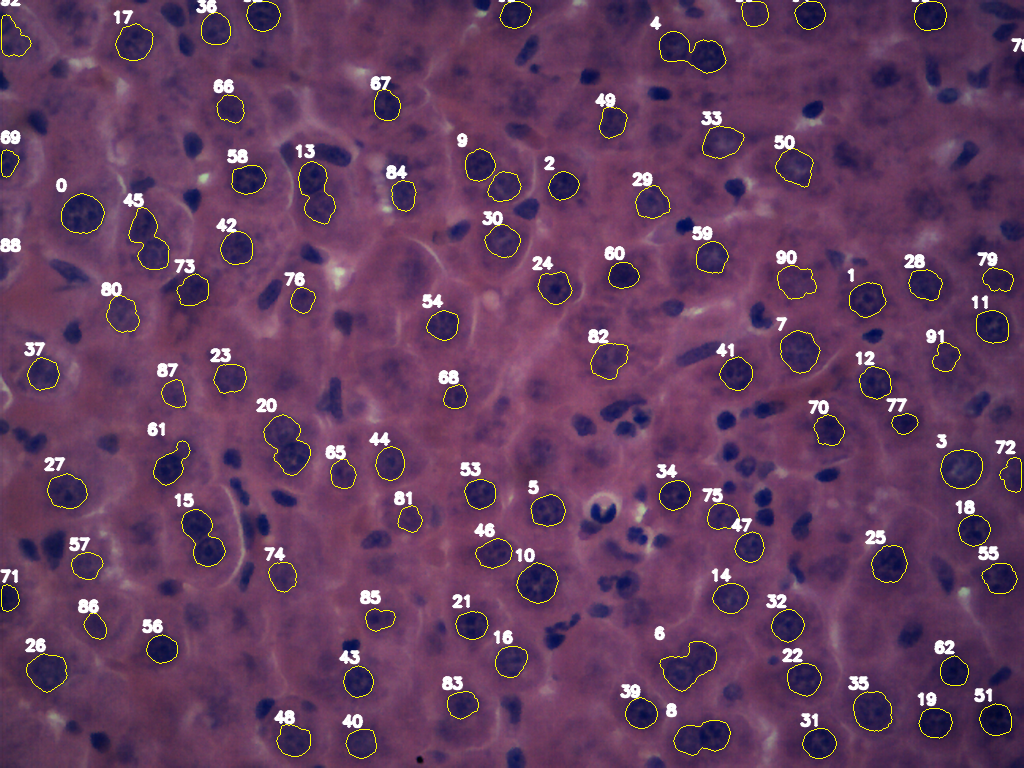
\includegraphics[width = 13cm, height = 9.8cm]{imagens_resultados/controle-seg-primeira.png}
    \caption{}
    \label{fig:controle-seg-primeira}
\end{figure}

\begin{figure}[!h]
    \centering
    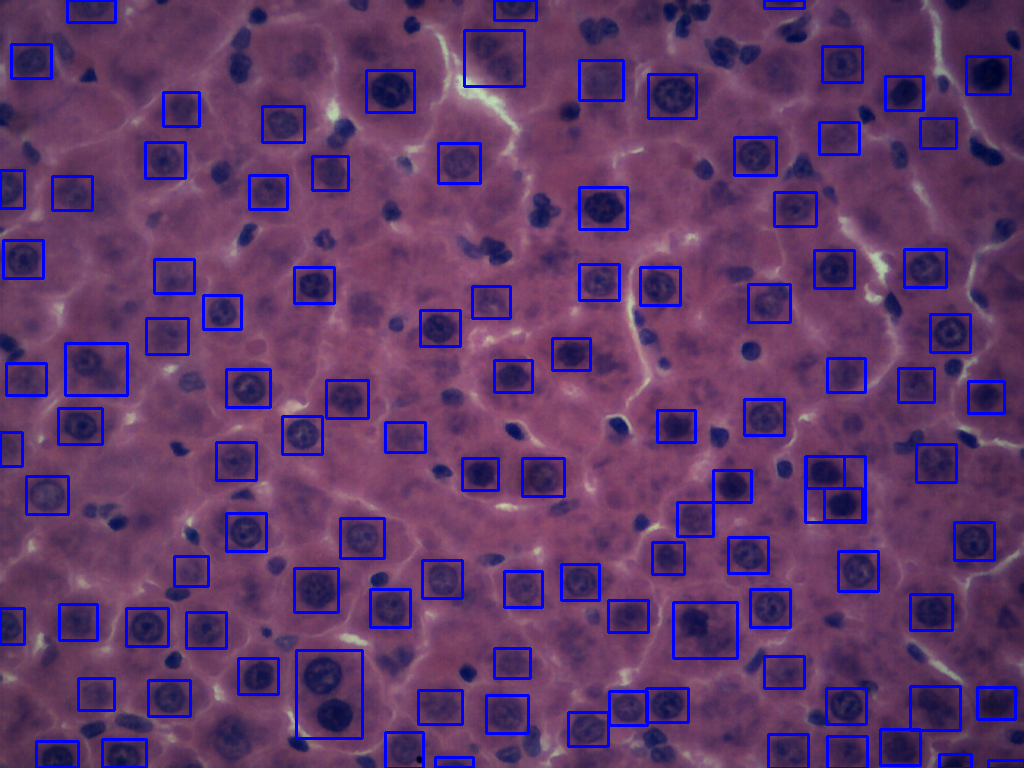
\includegraphics[width = 13cm, height = 9.8cm]{imagens_resultados/controle-yolo-segunda.png}
    \caption{Imagem resultante da YOLO.}
    \label{fig:controle-yolo-segunda}
\end{figure}

\begin{figure}[!h]
    \centering
    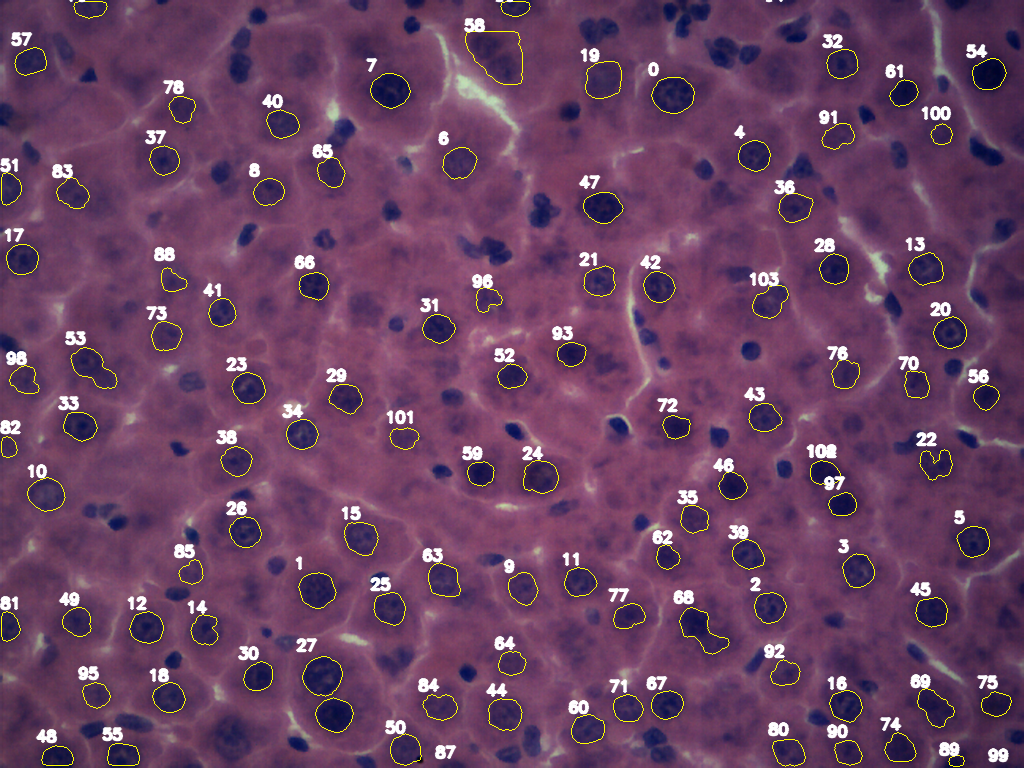
\includegraphics[width = 13cm, height = 9.8cm]{imagens_resultados/controle-seg-segunda.png}
    \caption{}
    \label{fig:controle-seg-segunda}
\end{figure}

\subsubsection{TW}

\begin{figure}[!h]
    \centering
    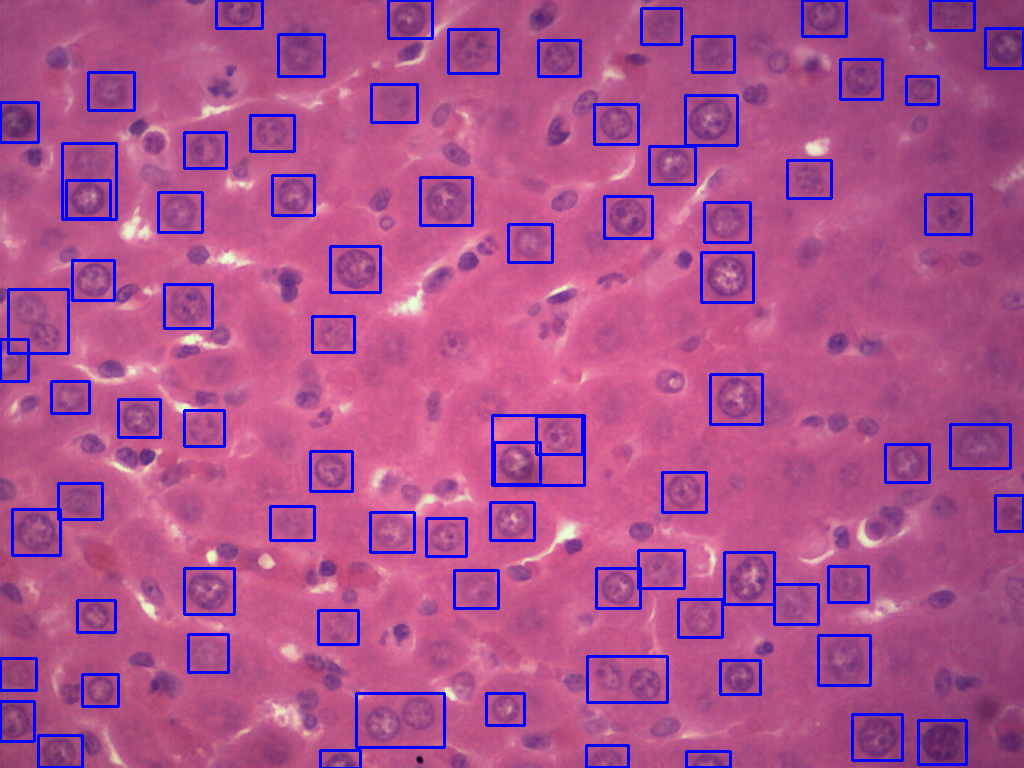
\includegraphics[width = 13cm, height = 9.8cm]{imagens_resultados/tw-yolo-primeira.png}
    \caption{Imagem resultante da YOLO.}
    \label{fig:tw-yolo-primeira}
\end{figure}

\begin{figure}[!h]
    \centering
    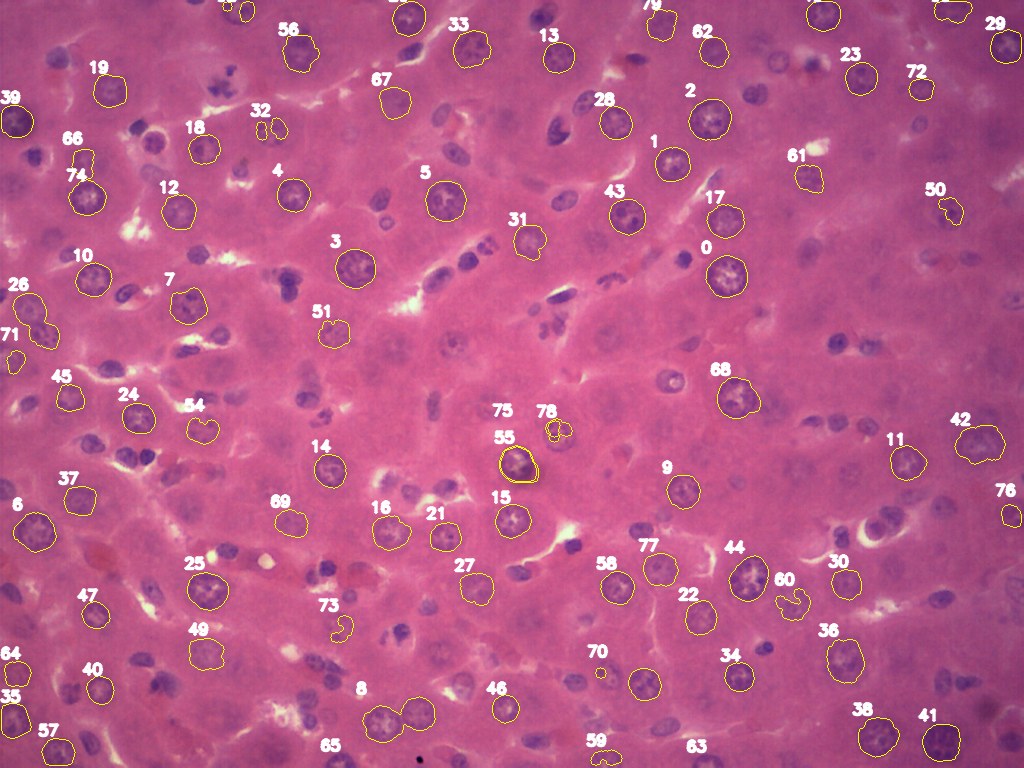
\includegraphics[width = 13cm, height = 9.8cm]{imagens_resultados/tw-seg-primeira.png}
    \caption{}
    \label{fig:tw-seg-primeira}
\end{figure}

\begin{figure}[!h]
    \centering
    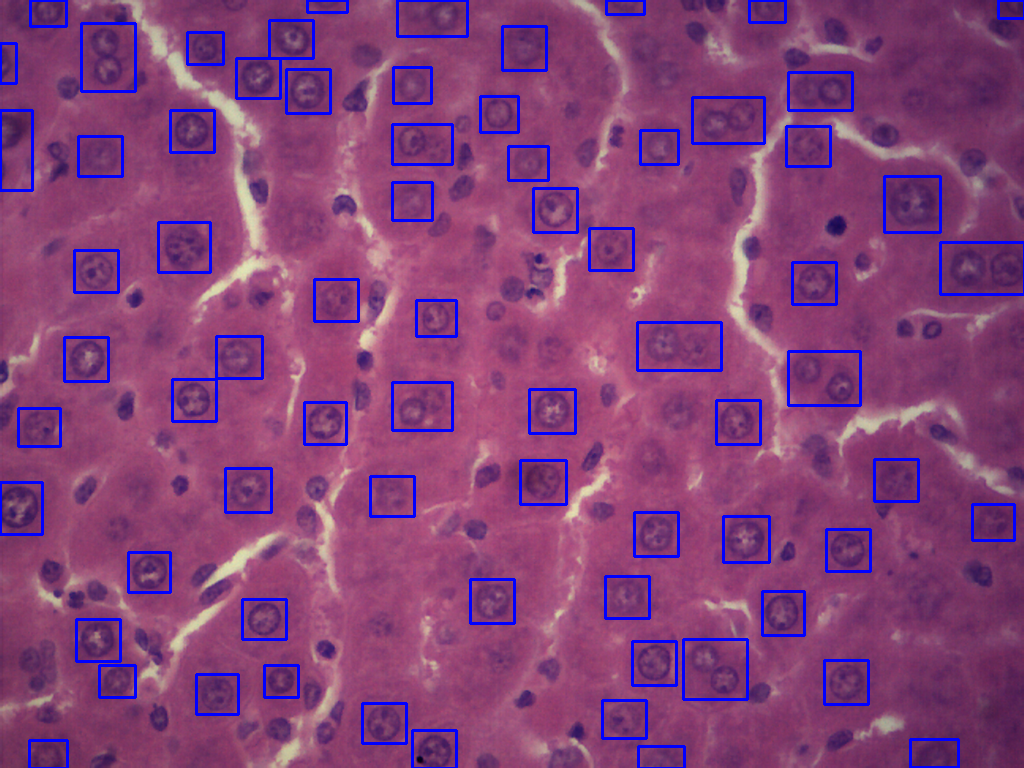
\includegraphics[width = 13cm, height = 9.8cm]{imagens_resultados/tw-yolo-segunda.png}
    \caption{Imagem resultante da YOLO.}
    \label{fig:tw-yolo-segunda}
\end{figure}

\begin{figure}[!h]
    \centering
    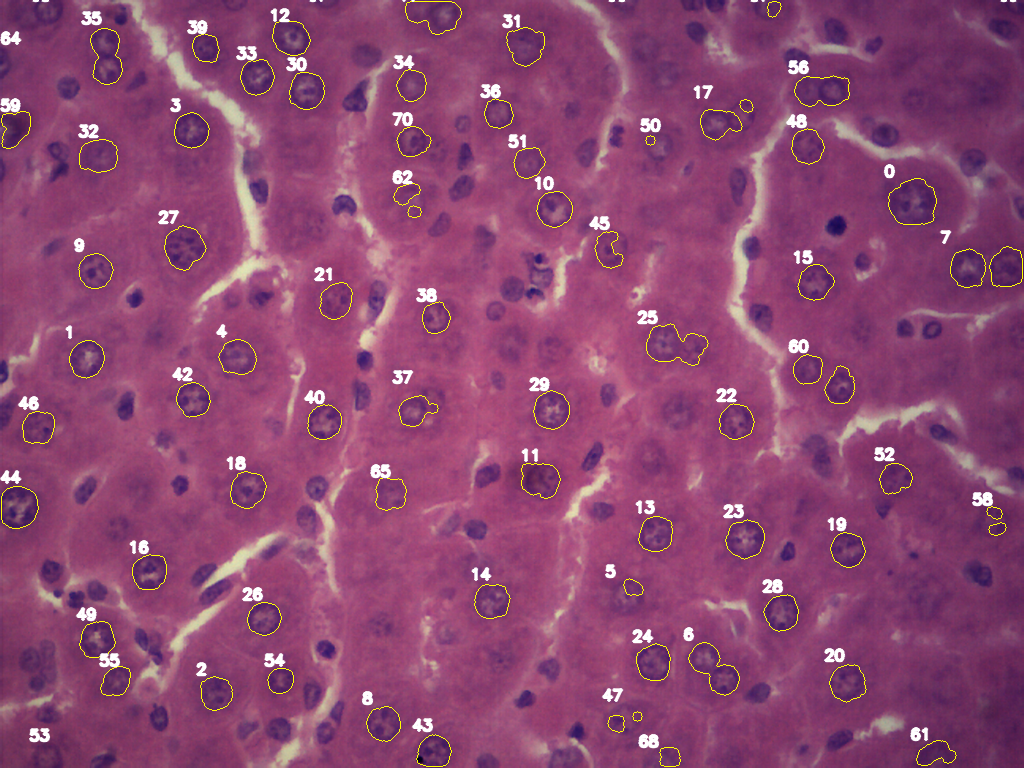
\includegraphics[width = 13cm, height = 9.8cm]{imagens_resultados/tw-seg-segunda.png}
    \caption{}
    \label{fig:tw-seg-segunda}
\end{figure}

\subsubsection{CONTROLE TRATADO}

\begin{figure}[!h]
    \centering
    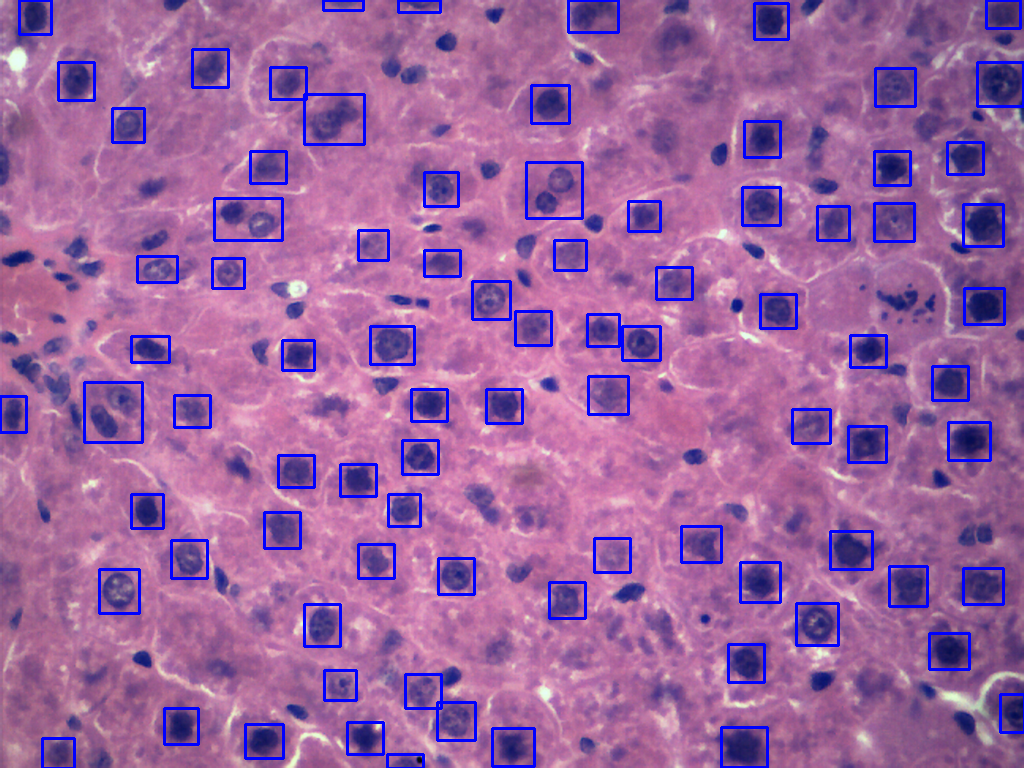
\includegraphics[width = 13cm, height = 9.8cm]{imagens_resultados/ct-yolo-primeira.png}
    \caption{Imagem resultante da YOLO.}
    \label{fig:ct-yolo-primeira}
\end{figure}

\begin{figure}[!h]
    \centering
    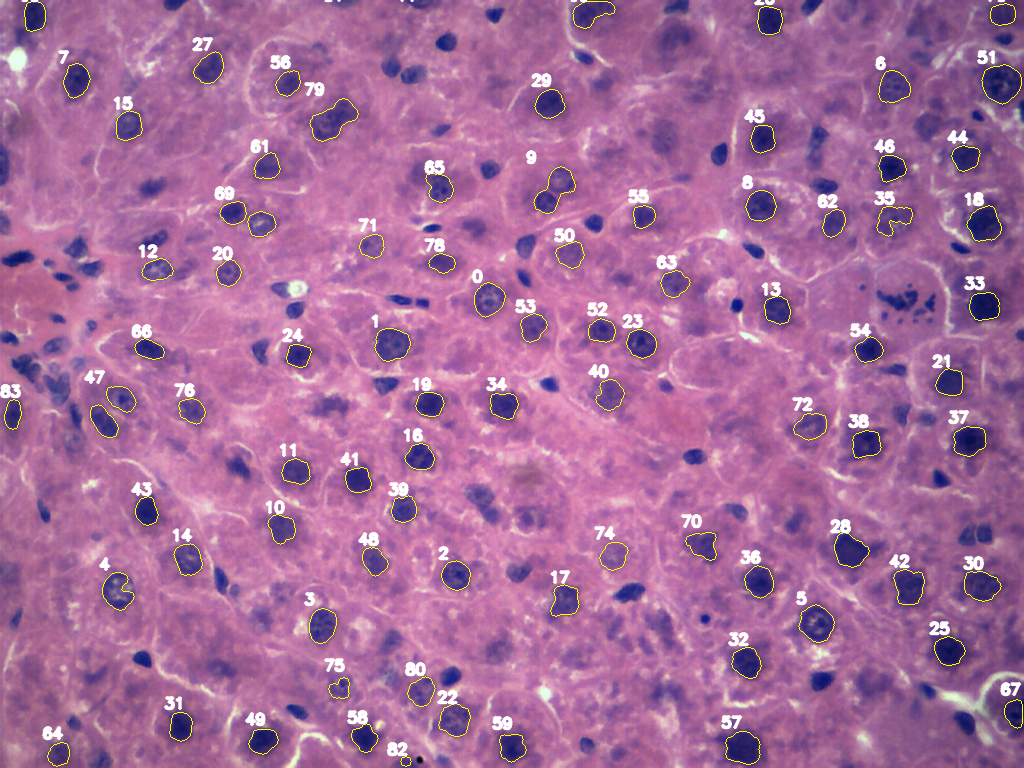
\includegraphics[width = 13cm, height = 9.8cm]{imagens_resultados/ct-seg-primeira.png}
    \caption{}
    \label{fig:ct-seg-primeira}
\end{figure}

\begin{figure}[!h]
    \centering
    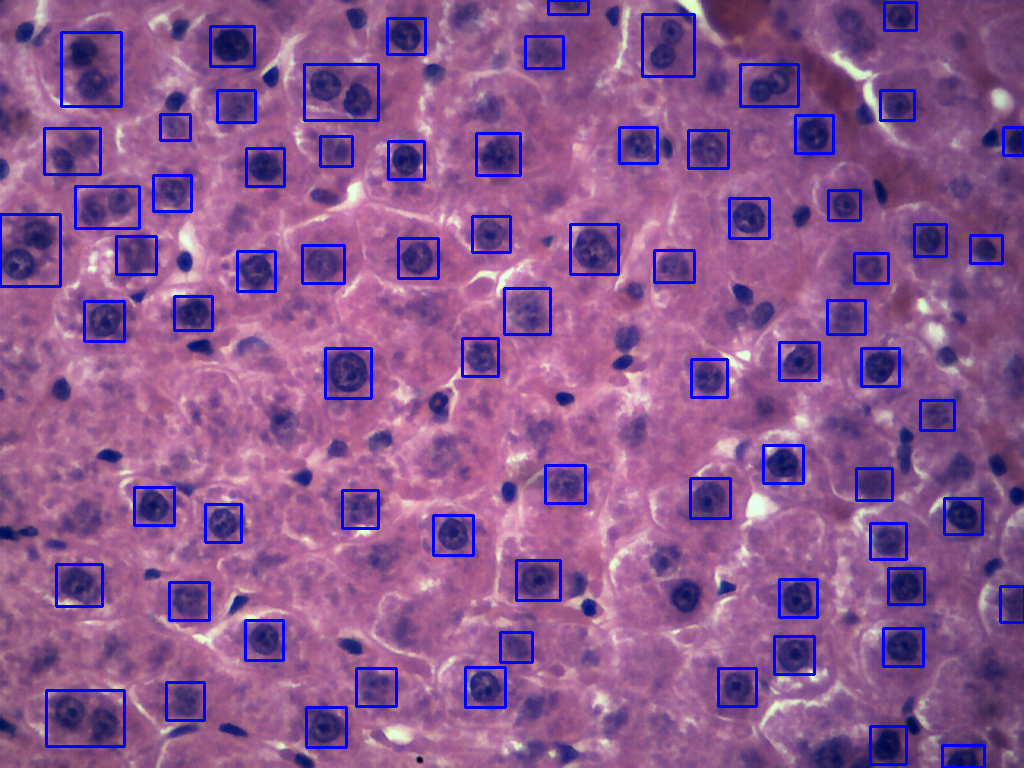
\includegraphics[width = 13cm, height = 9.8cm]{imagens_resultados/ct-yolo-segunda.png}
    \caption{Imagem resultante da YOLO.}
    \label{fig:ct-yolo-segunda}
\end{figure}

\begin{figure}[!h]
    \centering
    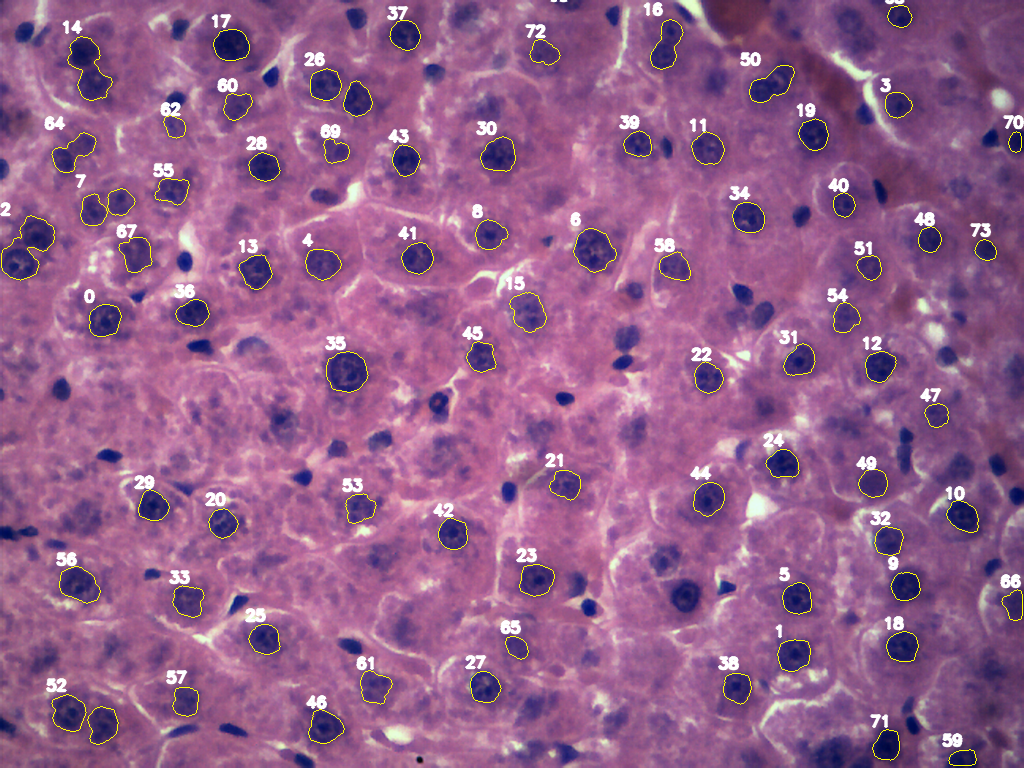
\includegraphics[width = 13cm, height = 9.8cm]{imagens_resultados/ct-seg-segunda.png}
    \caption{}
    \label{fig:ct-seg-segunda}
\end{figure}

\subsubsection{TW TRATADO}

\begin{figure}[!h]
    \centering
    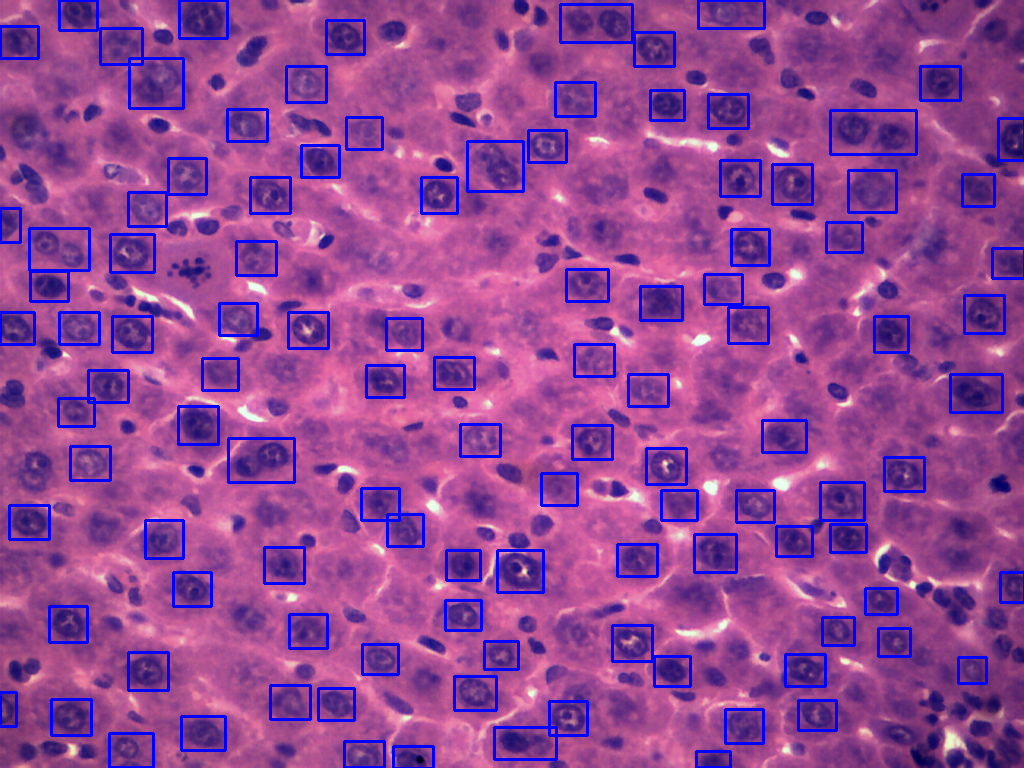
\includegraphics[width = 13cm, height = 9.8cm]{imagens_resultados/twt-yolo-primeira.png}
    \caption{Imagem resultante da YOLO.}
    \label{fig:twt-yolo-primeira}
\end{figure}

\begin{figure}[!h]
    \centering
    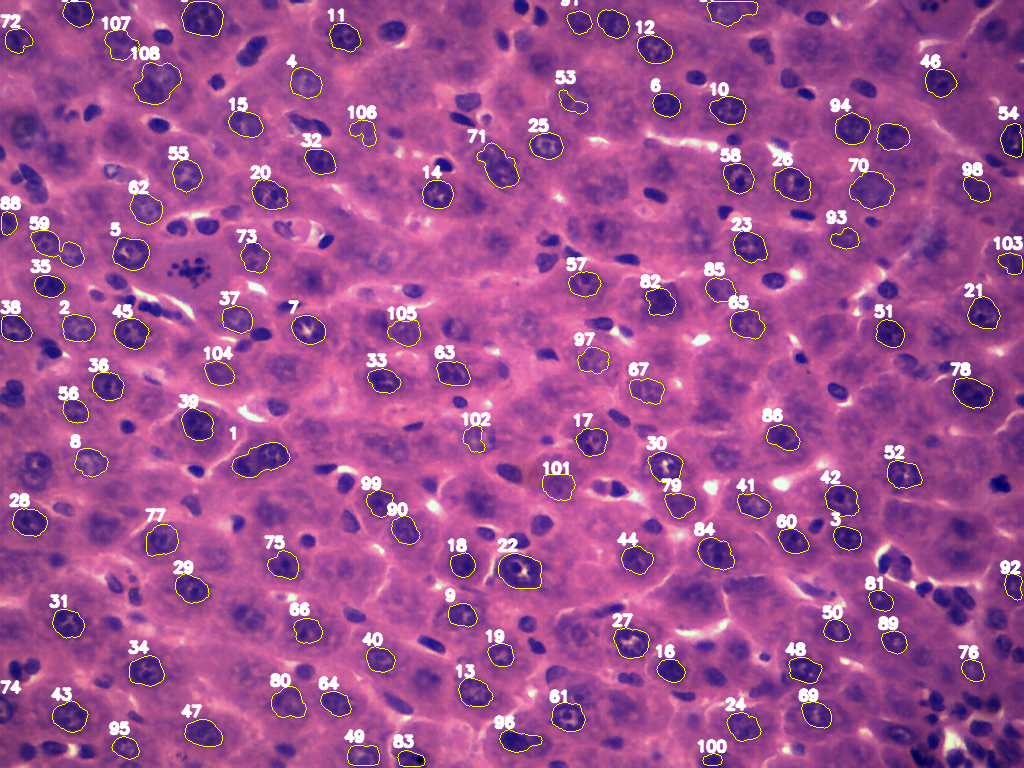
\includegraphics[width = 13cm, height = 9.8cm]{imagens_resultados/twt-seg-primeira.png}
    \caption{}
    \label{fig:twt-seg-primeira}
\end{figure}

\begin{figure}[!h]
    \centering
    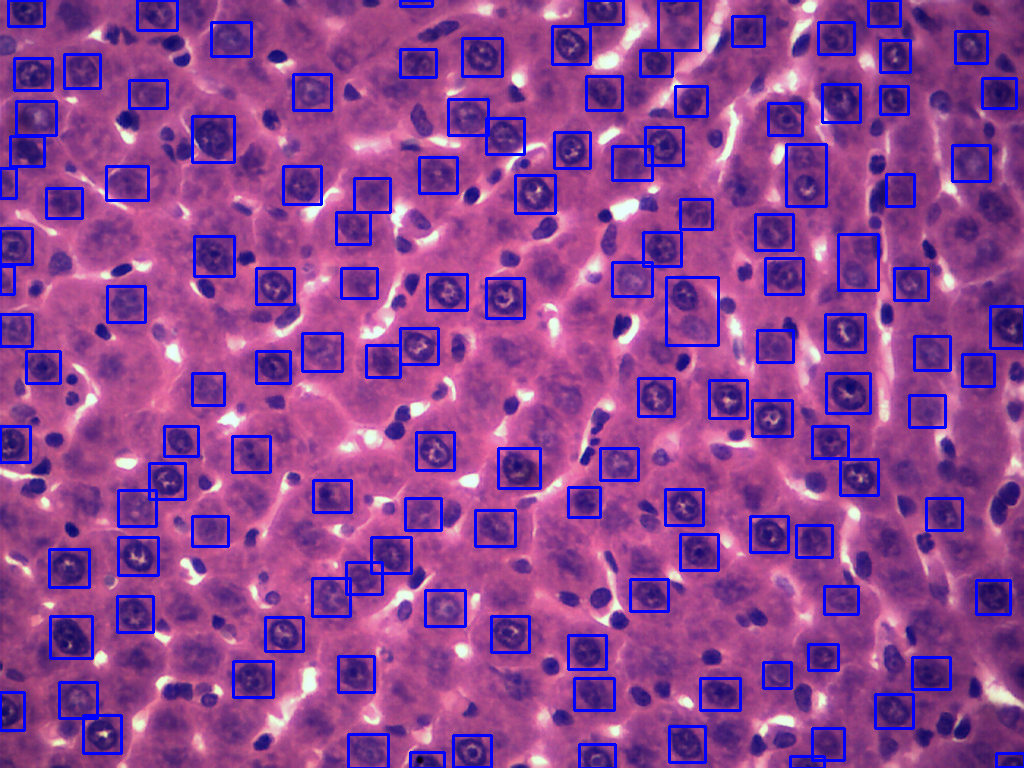
\includegraphics[width = 13cm, height = 9.8cm]{imagens_resultados/twt-yolo-segunda.png}
    \caption{Imagem resultante da YOLO.}
    \label{fig:twt-yolo-segunda}
\end{figure}

\begin{figure}[!h]
    \centering
    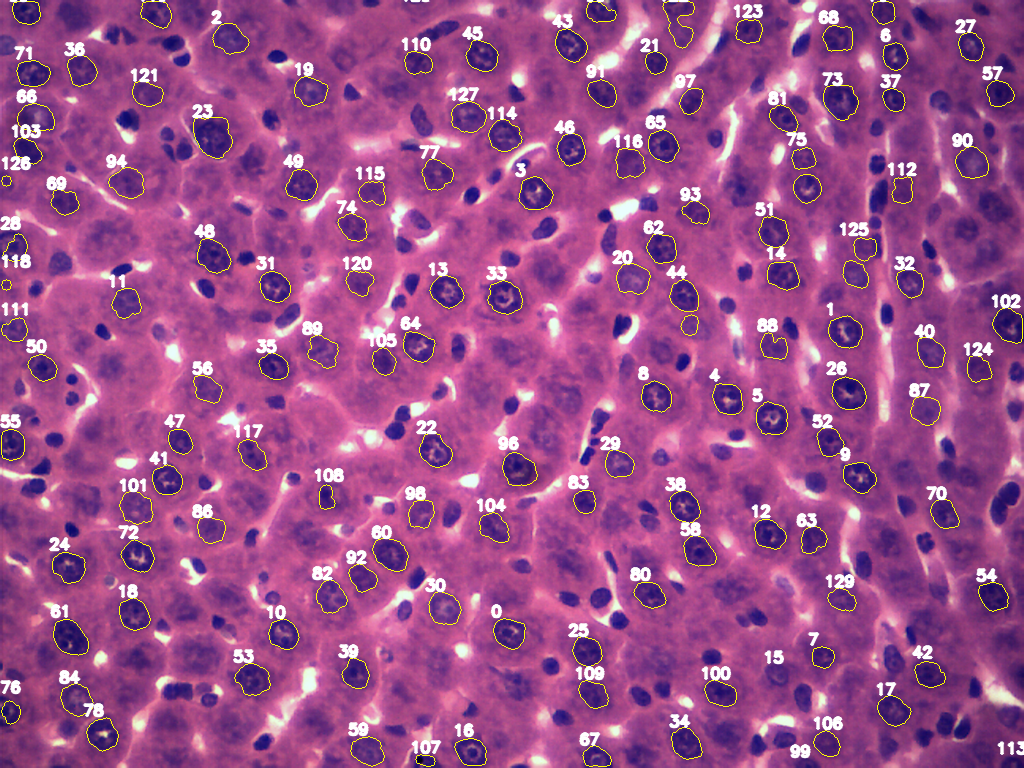
\includegraphics[width = 13cm, height = 9.8cm]{imagens_resultados/twt-seg-segunda.png}
    \caption{}
    \label{fig:twt-seg-segunda}
\end{figure}

Observando as figuras resultantes da YOLO é notado que todos os núcleos que há na imagem foram encontrados, isto é, sabemos quantos núcleos há na imagem que está sendo analisada. Por exemplo, na figura \ref{fig:tw-yolo-segunda} há 71 núcleos, na figura \ref{fig:twt-yolo-primeira} há 109 núcleos e na figura \ref{fig:ct-yolo-primeira} há 84 núcleos. No entanto, pode-se observar que na figura \ref{fig:tw-yolo-primeira} existem dois núcleos que são contados duas vezes o que implica em um erro na contagem da quantidade de núcleos, porém isso pode ser resolvido melhorando o treinamento da YOLO.

Os núcleos são enumerados, pois ao final do processo de segmentação é gerado uma tabela que contém a área e o perímetro de cada núcleo presente na imagem. A tabela \ref{tab:resultados-primeiro-metodo}\footnote{A tabela completa pode ser vista em \url{https://github.com/mafta-00/project_dissertacao/blob/fe22c3b183519a12434d9ceb73827a02ee8a9b00/dissertacao/capitulo_4\%20-\%20resultados/tabelas/primeira_tabela.csv}} é o resultado final da figura \ref{fig:twt-yolo-primeira}. Os valores de área e perímetro estão em pixel.

\begin{table}[h]
    \centering
    \caption{}
    \begin{tabular}{c|c|c|c|c|c|c|c|c}
        \hline
        Núcleo    & 0 & 1 & 2 & 3 & 4 & \dots & 107 & 108 \\
        \hline    
        Área      & 1236 & 1367 & 780 & 552 & 788 & \dots & 769 & 1469 \\
        \hline  
        Perímetro &  117 & 134 & 93 & 75 & 91 & \dots & 93 & 131 \\
        \hline
    \end{tabular}
    \label{tab:resultados-primeiro-metodo}
\end{table}

\subsection{SEGUNDO MÉTODO DE SEGMENTAÇÃO}

Agora, serão apresentados os resultados obtidos pelo segundo método de segmentação. As figuras \ref{fig:controle-yolo-primeira_2}, \ref{fig:controle-yolo-segunda_2}, \ref{fig:tw-yolo-primeira_2}, \ref{fig:tw-yolo-segunda_2}, \ref{fig:ct-yolo-primeira_2}, \ref{fig:controle-yolo-segunda_2}, \ref{fig:twt-yolo-primeira_2} e \ref{fig:twt-yolo-segunda_2} ilustra imagens depois da aplicação da função de mínimo local. Já as figuras \ref{fig:controle-seg-primeira_2}, \ref{fig:controle-seg-segunda_2}, \ref{fig:tw-seg-primeira_2}, \ref{fig:tw-seg-segunda_2}, \ref{fig:ct-seg-primeira_2}, \ref{fig:ct-seg-segunda_2}, \ref{fig:twt-seg-primeira_2} e \ref{fig:twt-seg-segunda_2} ilustram o resultado final do segundo método de segmentação. As imagens segmentadas foram obtidas utilizando os parâmetros $n = 13$ porque permitiu que os núcleos fossem preservados na imagem resultante, removendo adequadamente os ruídos e, também, limiar de circularidade igual $0.6$ pois é obtido uma quantidade boa de núcleos com este limiar.

\subsubsection{CONTROLE}

\begin{figure}[!h]
    \centering
    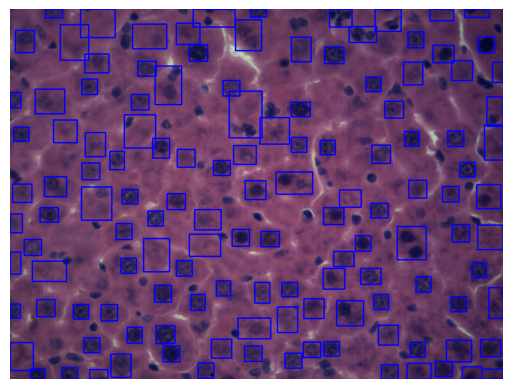
\includegraphics[width = 13cm, height = 9.8cm]{imagens_resultados/controle-yolo-primeira_2.png}
    \caption{Imagem resultante da YOLO.}
    \label{fig:controle-yolo-primeira_2}
\end{figure}

\begin{figure}[!h]
    \centering
    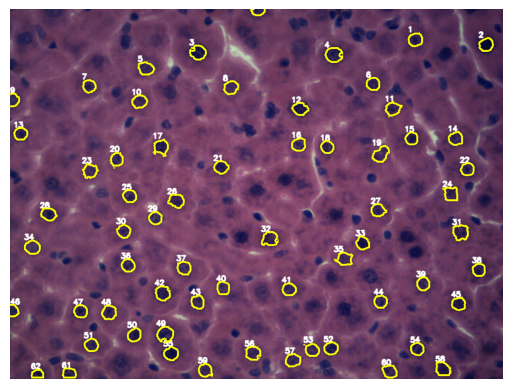
\includegraphics[width = 13cm, height = 9.8cm]{imagens_resultados/controle-seg-primeira_2.png}
    \caption{}
    \label{fig:controle-seg-primeira_2}
\end{figure}

\begin{figure}[!h]
    \centering
    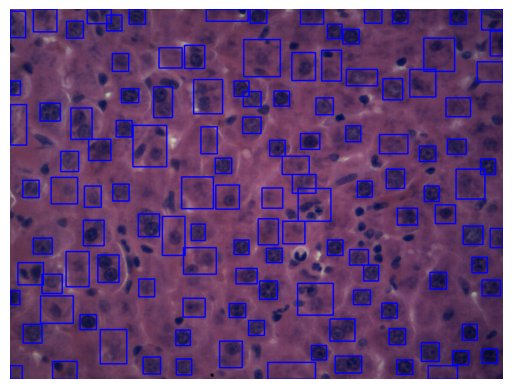
\includegraphics[width = 13cm, height = 9.8cm]{imagens_resultados/controle-yolo-segunda_2.png}
    \caption{Imagem resultante da YOLO.}
    \label{fig:controle-yolo-segunda_2}
\end{figure}

\begin{figure}[!h]
    \centering
    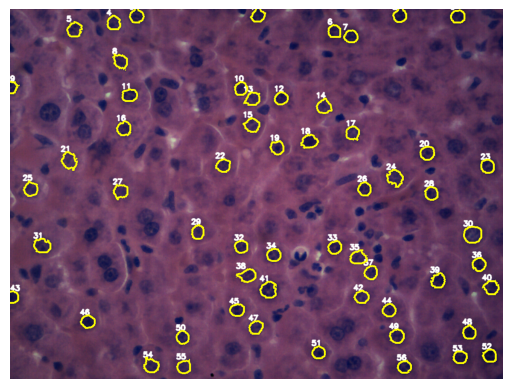
\includegraphics[width = 13cm, height = 9.8cm]{imagens_resultados/controle-seg-segunda_2.png}
    \caption{}
    \label{fig:controle-seg-segunda_2}
\end{figure}

\subsubsection{TW}

\begin{figure}[!h]
    \centering
    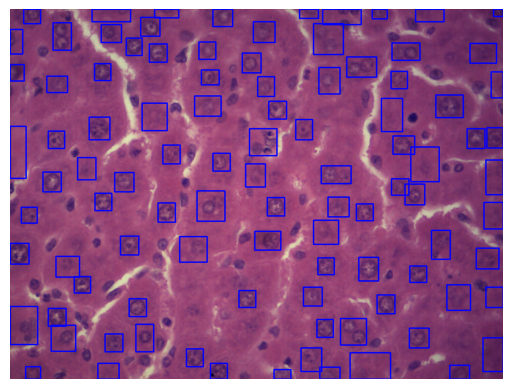
\includegraphics[width = 13cm, height = 9.8cm]{imagens_resultados/tw-yolo-primeira_2.png}
    \caption{Imagem resultante da YOLO.}
    \label{fig:tw-yolo-primeira_2}
\end{figure}

\begin{figure}[!h]
    \centering
    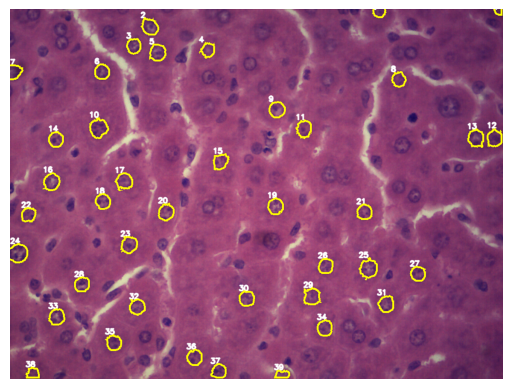
\includegraphics[width = 13cm, height = 9.8cm]{imagens_resultados/tw-seg-primeira_2.png}
    \caption{}
    \label{fig:tw-seg-primeira_2}
\end{figure}

\begin{figure}[!h]
    \centering
    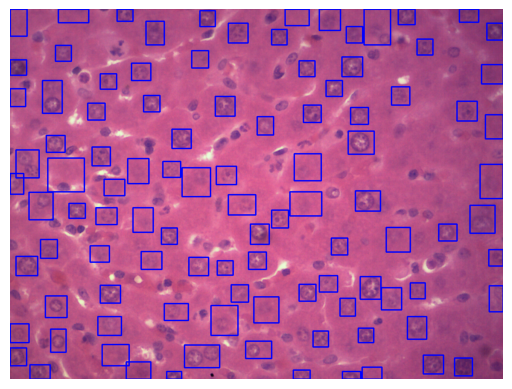
\includegraphics[width = 13cm, height = 9.8cm]{imagens_resultados/tw-yolo-segunda_2.png}
    \caption{Imagem resultante da YOLO.}
    \label{fig:tw-yolo-segunda_2}
\end{figure}

\begin{figure}[!h]
    \centering
    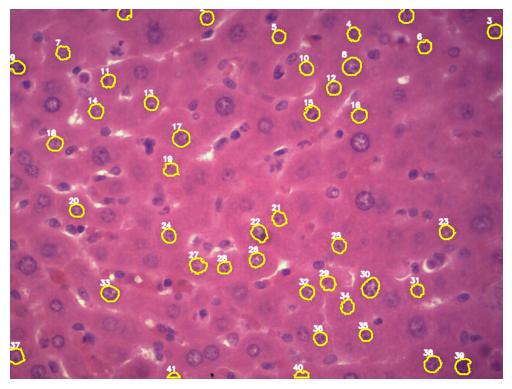
\includegraphics[width = 13cm, height = 9.8cm]{imagens_resultados/tw-seg-segunda_2.png}
    \caption{}
    \label{fig:tw-seg-segunda_2}
\end{figure}

\subsubsection{CONTROLE TRATADO}

\begin{figure}[!h]
    \centering
    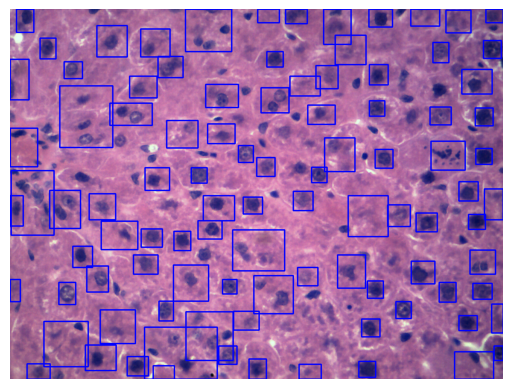
\includegraphics[width = 13cm, height = 9.8cm]{imagens_resultados/ct-yolo-primeira_2.png}
    \caption{Imagem resultante da YOLO.}
    \label{fig:ct-yolo-primeira_2}
\end{figure}

\begin{figure}[!h]
    \centering
    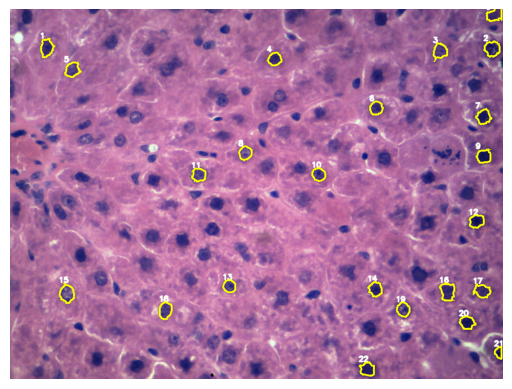
\includegraphics[width = 13cm, height = 9.8cm]{imagens_resultados/ct-seg-primeira_2.png}
    \caption{}
    \label{fig:ct-seg-primeira_2}
\end{figure}

\begin{figure}[!h]
    \centering
    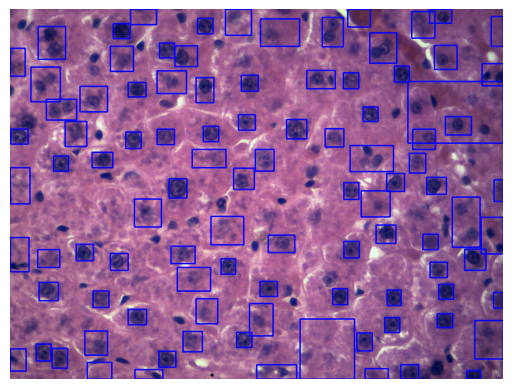
\includegraphics[width = 13cm, height = 9.8cm]{imagens_resultados/ct-yolo-segunda_2.png}
    \caption{Imagem resultante da YOLO.}
    \label{fig:ct-yolo-segunda_2}
\end{figure}

\begin{figure}[!h]
    \centering
    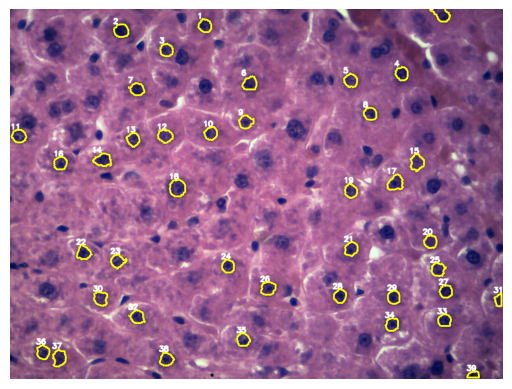
\includegraphics[width = 13cm, height = 9.8cm]{imagens_resultados/ct-seg-segunda_2.png}
    \caption{}
    \label{fig:ct-seg-segunda_2}
\end{figure}

\subsubsection{TW TRATADO}

\begin{figure}[!h]
    \centering
    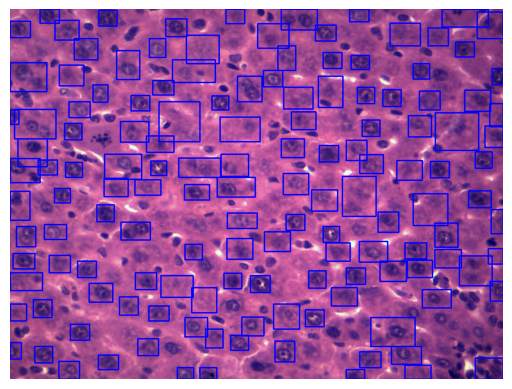
\includegraphics[width = 13cm, height = 9.8cm]{imagens_resultados/twt-yolo-primeira_2.png}
    \caption{Imagem resultante da YOLO.}
    \label{fig:twt-yolo-primeira_2}
\end{figure}

\begin{figure}[!h]
    \centering
    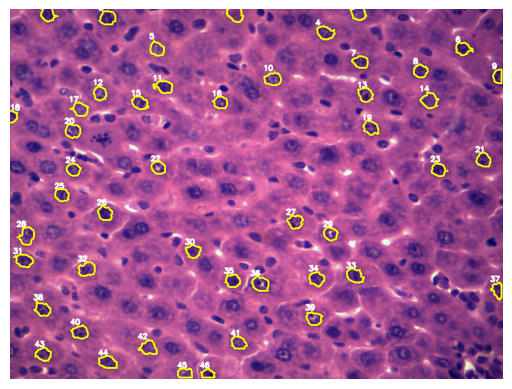
\includegraphics[width = 13cm, height = 9.8cm]{imagens_resultados/twt-seg-primeira_2.png}
    \caption{}
    \label{fig:twt-seg-primeira_2}
\end{figure}

\begin{figure}[!h]
    \centering
    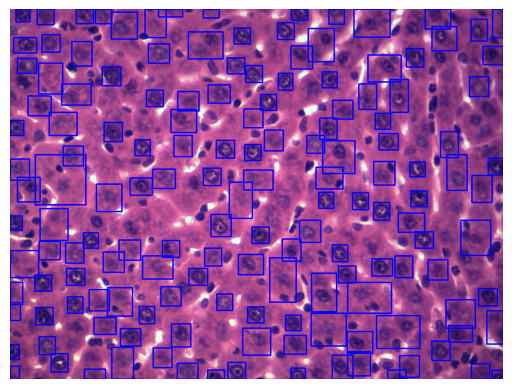
\includegraphics[width = 13cm, height = 9.8cm]{imagens_resultados/twt-yolo-segunda_2.png}
    \caption{Imagem resultante da YOLO.}
    \label{fig:twt-yolo-segunda_2}
\end{figure}

\begin{figure}[!h]
    \centering
    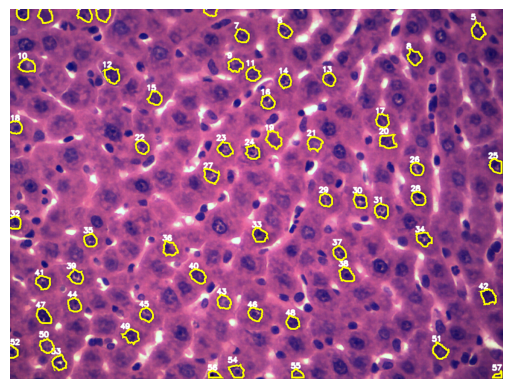
\includegraphics[width = 13cm, height = 9.8cm]{imagens_resultados/twt-seg-segunda_2.png}
    \caption{}
    \label{fig:twt-seg-segunda_2}
\end{figure}

Analisando as figuras resultante do método de mínimo local é observado que a maioria dos núcleos que há na imagem foram encontrados, no entanto muitos ruídos também foram encontrados, implicando que é necessário fazer uma filtragem para obter a quantidade de núcleos que a imagem possui. Uma filtragem possível é identificar os núcleos pelo valor de sua circularidade, como foi realizado neste trabalho. Com isso, é notado que uma boa parte dos núcleos são segmentados corretamente e uma outra parte é descartada.

Os núcleos são enumerados, pois ao final do processo de segmentação é gerado uma tabela que contém a área e o perímetro de cada núcleo presente na imagem. A tabela \ref{tab:resultados-segundo-metodo}\footnote{A tabela completa pode ser vista em \url{https://github.com/mafta-00/project_dissertacao/blob/c3be1aeef23fc6a94b59ea4270ffaa8013d2ea25/dissertacao/capitulo_4\%20-\%20resultados/tabelas/segunda_tabela.csv}} é o resultado final da figura \ref{fig:ct-seg-primeira_2}. Os valores de área e perímetro estão em pixel.

\begin{table}[h]
    \centering
    \caption{}
    \begin{tabular}{c|c|c|c|c|c|c|c|c}
        \hline
        Núcleo    &  0 & 1 & 2 & 3 & 4 & \dots & 21 & 22\\
        \hline    
        Área      &  811 & 927 & 985 & 890 & 729 & \dots & 428 & 834 \\
        \hline  
        Perímetro & 128.462 & 137.847 & 132.054 & 135.539 & 104.983 & \dots & 83.4558 & 123.225 \\
        \hline
    \end{tabular}
    \label{tab:resultados-segundo-metodo}
\end{table}

\subsection{TESTE REALIZADO}

Para avaliar adequadamente os resultados, foi comparado os núcleos segmentados pelos métodos proposto com o \textit{ground truth}, isto é, uma máscara de segmentação feita manualmente pelos pesquisadores do Laboratório de Plasticidade Neural Entérica. Foram feitas 80 imagens de \textit{ground truth} com 15 núcleos cada, uma vez que o processo de segmentação manual é extremamente cansativo. A figura \ref{fig:mascara_manual} ilustra algumas máscaras \textit{ground truth} feitas manualmente pelos pesquisadores do Laboratório de Plasticidade Neural Entérica.

\begin{figure}[!h]
    \centering
    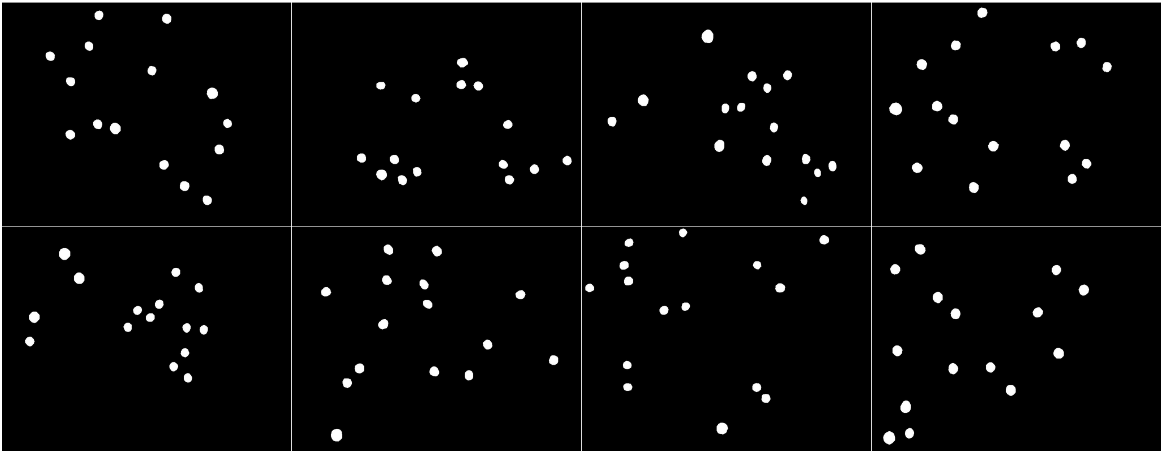
\includegraphics[width = 16cm, height = 6.25cm]{imagens_resultados/mascara_manual.png}
    \caption{Máscaras \textit{ground truth}.}
    \label{fig:mascara_manual}
\end{figure}

No processo de comparação, utilizou-se a métrica \textit{Intersection over Union} (IoU) na qual os valores produzidos variam de 0 a 1 (0–100\%), sendo que quanto maior o valor, maior a sobreposição entre duas regiões comparadas, $reg_1$ e $reg_2$. Matematicamente, a métrica IoU é expressa como

\begin{equation}
	\textrm{IoU} = \frac{\mathcal{A}(\mathtt{reg_1 \cap reg_2})}{\mathcal{A}(\mathtt{reg_1\cup reg_2})}.
	\label{eq:IoU}
\end{equation}

A tabela \ref{tab:resultados-geral} mostra o IoU médio para as técnicas de segmentação realizadas nas 80 imagens o

\begin{table}[h]
    \centering
    \caption{}
    \begin{tabular}{c|c}
        \hline
        \textbf{COMPARAÇÕES} & \textbf{IoU} \\
        \hline    
        ASF–REC ABE $\rightarrow$ FEC vs \textit{ground truth} & \textbf{0.8823}\\
        \hline  
        ASF–REC FEC $\rightarrow$ ABE \textit{ground truth} & 0.8789\\
        \hline
        ASF–REC ABE $\rightarrow$ FEC vs YOLOv8 & 0.8759\\
        \hline
        ASF–REC FEC $\rightarrow$ ABE vs YOLOv8 & 0.8731\\
        \hline
        \textit{ground truth} vs YOLOv8 & 0.8636\\
        \hline
        ASF–REC ABE $\rightarrow$ FEC vs ASF–REC FEC $\rightarrow$ ABE & 0.9932 \\
        \hline
    \end{tabular}
    \label{tab:resultados-geral}
\end{table}

Como é visto, quando comparado com a \textit{ground truth}, o melhor resultado foi obtido usando a segunda técnica de segmentação utilizando, \textbf{ASF–REC ABE $\rightarrow$ FEC}. Além disso, a comparação entre ASF–REC FEC $\rightarrow$ ABE e ASF–REC ABE $\rightarrow$ FEC obteve um IoU muito alto, 99.32\%, considerando que ambas estratégias fornecem resultados bastante semelhantes. É importante destacar que esses resultados, tanto para ASF–REC FEC $\rightarrow$ ABE quanto para ASF–REC ABE $\rightarrow$ FEC, foram obtidos usando $n=13$. 
\end{document}
